\documentclass[aspectratio=43]{beamer}
\usepackage[latin1]{inputenc}
\usepackage{amsmath}
\usepackage{amsfonts}
\usepackage{amssymb}
\usepackage{makeidx}
\usepackage{graphicx}
\usepackage{array}

% Customization
\mode<presentation>{
\usetheme{CambridgeUS}
\usecolortheme{dolphin}
\setbeamertemplate{navigation symbols}{}
}

% Define colors
\definecolor{darkgreen}{rgb}{0.0, 0.5, 0.13}
\definecolor{darkblue}{rgb}{0.0, 0.0, 0.55}
\definecolor{darkred}{rgb}{0.55, 0.0, 0.0}

%************************************************************************************************************

% Title and author
\title[QCD and Monte Carlo]{QCD and Monte Carlo}
\author{\textbf {Jes\'us Urtasun Elizari}}
\date{Milan, February 2021}

\begin{document}

% Front slide
\begin{frame}
	
	%\maketitle
	\vspace{1.0 cm}
	
	\center{\color{blue}QCD and Monte Carlo event generators}
	
	\vspace{0.25 cm}
	\center{Monte Carlo course seminar - Milan, February 2021}

	\begin{figure}
		\minipage{1\textwidth}
		
\includegraphics[width = 3.0 cm]{plots/logo_unimi.png}
		\hfill
		
\includegraphics[width = 3.0 cm]{plots/logo_infn.png}
		\hfill
		
\includegraphics[width = 3.0 cm]{plots/logo_erc.png}
		\endminipage
	\end{figure}

	\vspace{1.0 cm}

\end{frame}

% Introduction
\begin{frame}

	\frametitle{Outline}
	
	\begin{enumerate}
		\item {\color{blue}Hadron collisions and strong interactions}
		\begin{itemize}
			\item Hadron collisions and strong interactions
			\item Renormalization group
			\item IR divergences
		\end{itemize}
		\item {\color{blue}MC and Parton Showers}
		\begin{itemize}
			\item Factorization theorem
			\item Final state radiation
			\item Initial state radiation
		\end{itemize}
		\item {\color{blue}Hadronization: some basics}
	\end{enumerate}
	
\end{frame}

% Strong interactions I
\begin{frame}

	\frametitle{Strong interactions}
	\framesubtitle{QCD from $e^{+}e^{-}$ annihilation}

	Quantum Chromodynamics (QCD) $\rightarrow$ theory describing the interaction between quarks and gluons (strong interactions)
	\begin{figure}
		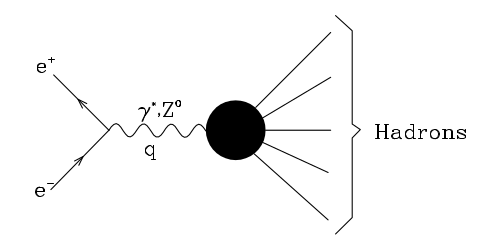
\includegraphics[width = 5 cm]{plots/ee_hadrons.png}
	\end{figure}
 
	QCD arises already from $e^{+}e^{-}$ annihilation $\rightarrow R_{0}$ ratio

	\begin{columns}
	
		\column{0.5\textwidth}
	
		\begin{figure}
			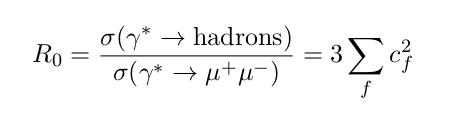
\includegraphics[width = 6 cm]{plots/eq_R0.png}
		\end{figure}
	
		\column{0.5\textwidth}
	
		\begin{enumerate}
			\item \footnotesize Color factor (3 color for each quark)
			\item \footnotesize Sum over charges of different flavors
			\item \footnotesize Threshold and higher order corrections
		\end{enumerate}	

	\end{columns}

\end{frame}

% Strong interactions II
\begin{frame}

	\frametitle{Strong interactions}
	\framesubtitle{QCD from $e^{+}e^{-}$ annihilation}
	
	Higher order corrections to $R_{0}$ 
	\begin{figure}
		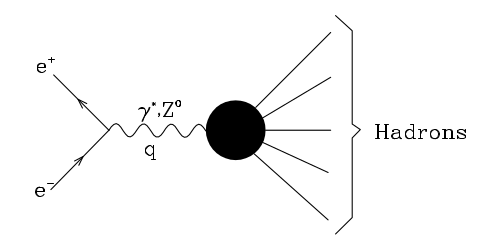
\includegraphics[width = 5 cm]{plots/ee_hadrons.png}
	\end{figure}
	
	QCD arises already from $e^{+}e^{-}$ annihilation $\rightarrow R_{0}$ ratio
	
	\begin{figure}
		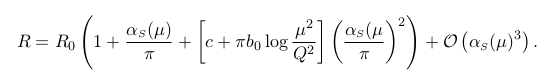
\includegraphics[width = 8 cm]{plots/eq_R0_3.png}
	\end{figure}

	\footnotesize $\alpha_{s}$ correction completely finite (IR cancellation) \\
	\footnotesize $\alpha_{s}^{2}$, UV divergences arise (Renormalization)
	
\end{frame}

% Renormalization group I
\begin{frame}

	\frametitle{Strong interactions}
	\framesubtitle{Renormalization group}
	
	\begin{itemize}
		\item Running coupling given by Renormalization Group Equation (RGE)
		\begin{equation}
			{\color{blue}\mu\frac{d\alpha_{s}(\mu)}{d\mu} = \beta(\alpha_{s}(\mu)) = -\sum_{n = 0}^{\infty} \beta_{n} \Big( \frac{\alpha_{s}}{\pi} \Big)^{n + 1}} \nonumber
		\end{equation}
		\item Coupling {\color{blue}$\alpha_{s}$} evolves with scale {\color{blue}$\mu$} as given by RGE $\rightarrow$ LO behavior driven by $\beta_{0}$
		\item $\beta_{0}^{\textrm{QCD}} > 0 \implies$ weakly coupled at large energies, asymptotic freedom
		\item $\beta_{0}^{\textrm{QED}} < 0 \implies$ strongly coupled at large energies, UV divergent!	
	\end{itemize}

\end{frame}

% Renormalization group II
\begin{frame}

	\frametitle{Strong interactions}
	\framesubtitle{Renormalization group}

	\begin{columns}	
	
		\column{0.5\textwidth}
		
		\begin{figure}
			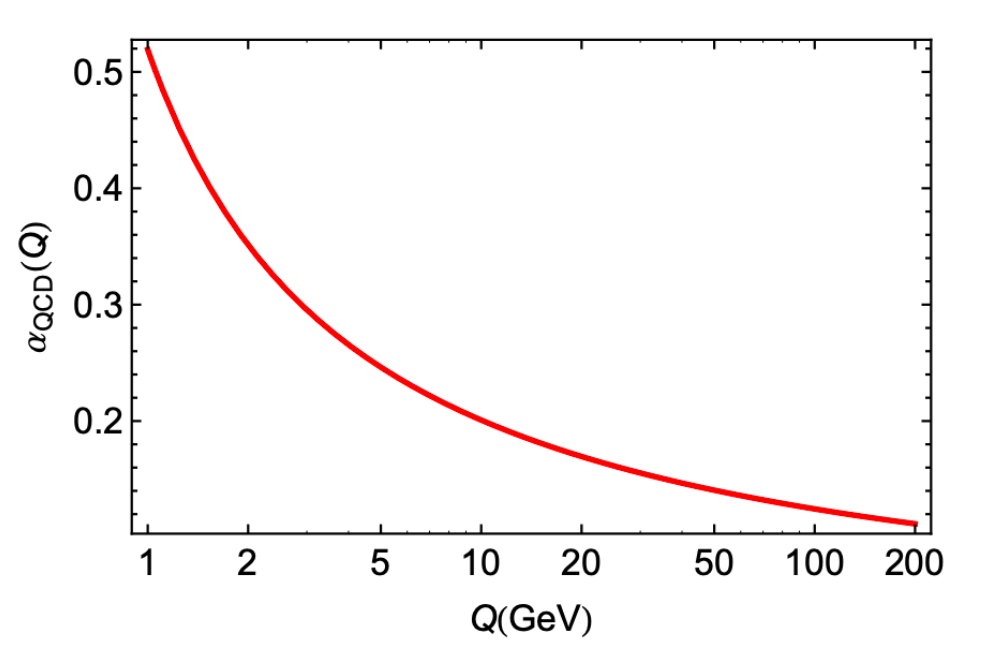
\includegraphics[width = 5 cm]{plots/qcd_coupling.png}
		\end{figure}

		\column{0.5\textwidth}
	
		\begin{itemize}
			\item \footnotesize Running coupling given by Renormalization Group Equation (RGE)
			\begin{equation}
				\alpha_{s}(\mu) = \frac{1}{\beta_{0} \log\big( \frac{\mu^{2}}{\Lambda_{s}^{2}}\big)} \nonumber
			\end{equation}
			\item \footnotesize $\beta_{0}$ LO of the $\beta$ function, is $ > 0$
			\item \footnotesize $\Lambda_{s}$, parameter that defines value of the coupling at large scales
		\end{itemize}

	\end{columns}
	
	\vspace{1cm}
	\center QCD is weakly coupled for $\mu >> \Lambda_{s} \longrightarrow$ asymptotically free
	\center \color{red} Perturbative Quantum Chromodynamics (pQCD)

\end{frame}

% Factorization theoren
\begin{frame}

	\frametitle{Factorization theorem}
	\framesubtitle{QCD factorization}
	
	\center \footnotesize LHC processes $H_{1} + H_{2} \rightarrow \textrm{F}$	
	\begin{figure}
		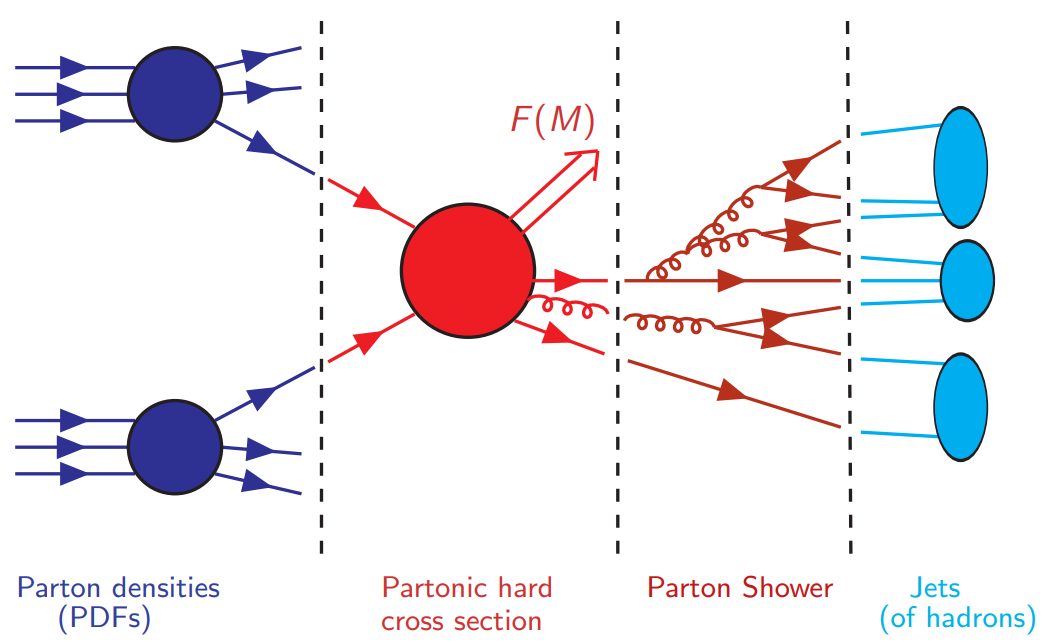
\includegraphics[width = 7 cm]{plots/factorization_1.png}
	\end{figure}
	
	\footnotesize {Separate process {\color{blue}PDFs} and {\color{red} partonic (hard) interaction}	
	\begin{equation}
		\sigma^{\textrm{F}}(p_{1}, p_{2}) = \sum_{\alpha, \beta}
		\int_{0}^{1} dx_{1} dx_{2} \; {\color{blue} f_{\alpha}(x_{1}, \mu_{F}^{2}) \ast f_{\beta}(x_{2}, \mu_{F}^{2})}
		\; \ast \;  
		{\color{red}\hat{\sigma}^{\textrm{F}}_{\alpha \beta}(x_{1}p_{1}, x_{2}p_{2}, \alpha_{s}(\mu_{R}^{2}), \mu_{F}^{2})} \nonumber
	\end{equation}}
		
\end{frame}

% Parton showers I
\begin{frame}

	\frametitle{Parton showers}
	\framesubtitle{MC Parton showers}
	
	\footnotesize Partons in the initial and final state emit radiation. Initial state Radiation (ISR) and Final State Radiation (FSR) model by Monte Carlo (MC) shower algorithms
	
	\vspace{0.1 cm}
	\center \color{red} Shower Monte Carlo programs (HERWIG, PYTHIA)
	\vspace{0.15 cm}
	
	\begin{itemize} 
		\item Libraries for computing SM and BSM cross sections
		\item Shower algorithms produce a number of enhanced
		coloured parton emissions \\
		to be added to the hard process
		\item Hadronization models, underlying event, decays of unstable hadrons, etc
	\end{itemize}

\end{frame}

% Parton showers II
\begin{frame}

	\frametitle{Parton showers}
	\framesubtitle{Collinear limit}
	
	\begin{itemize} 
		\item \footnotesize QCD emission processes are enhanced in the collinear limit ($\theta$ small)
		\item \footnotesize $\sigma$ dominated by collinear splittings $q \rightarrow qg, g \rightarrow gg, g \rightarrow q\bar{q}$ \\
		(measurement not sensitive to such small scales)
	\end{itemize}
	
	\begin{figure}
		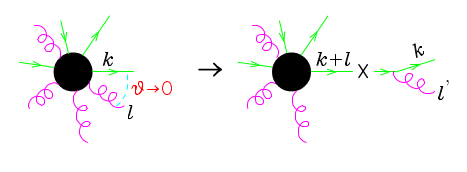
\includegraphics[width = 6 cm]{plots/collinear_factorization.png}
	\end{figure}
	
	\footnotesize Collinear factorization $\longrightarrow$ The cross section factorizes
	into the product of a tree-level cross section and a splitting
	factorFactor out tree level amplitude and splitting
	\begin{figure}
		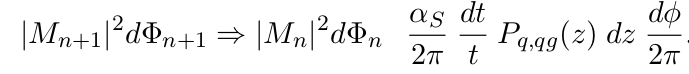
\includegraphics[width = 7 cm]{plots/eq_factorization_theorem.png}
	\end{figure}

	\begin{figure}
		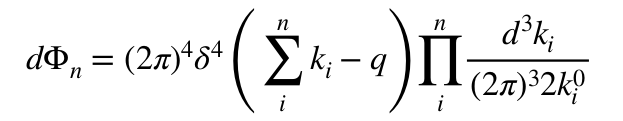
\includegraphics[width = 5 cm]{plots/eq_factorization_ps.png}
	\end{figure}

\end{frame}

% Parton showers III
\begin{frame}

	\frametitle{Parton showers}
	\framesubtitle{Kinematics of splitting}
	
	\begin{figure}
		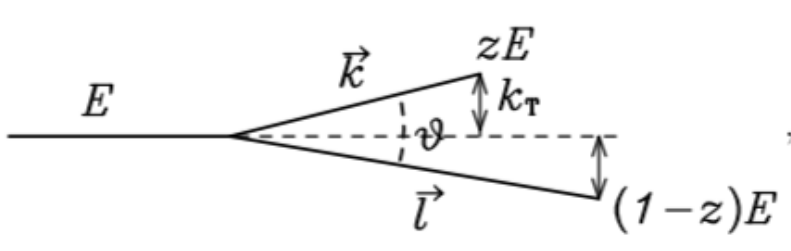
\includegraphics[width = 5 cm]{plots/shower_kinematics.png}
	\end{figure}
	
	\footnotesize Kinematics of splitting given by $(t, z, \phi)$
	\begin{itemize}
		\item $t$: parameter with dimensions of energy that vanish in the collinear limit \\
		\begin{itemize}
			\item Virtuality $t = (k + l)^{2} = k^{0}l^{0}4\sin^{2}\bigg( \frac{\theta}{2} \bigg) \approx k^{0}l^{0}\theta^{2} \approx z(1 - z)E^{2}\theta^{2}$
			\item Transverse momentum $t = k_{\perp}^{2} = l_{\perp}^{2} = z^{2}(1 - z)^{2}E^{2}\theta^{2}$
			\item Hardness $E^{2}\theta^{2}$
		\end{itemize}
		\item $z$: fraction of energy of radiated parton $z = \frac{k^{0}}{k^{0} + l^{0}}$
		\item $\phi$ represents azimuth of the $k, l$ plane
	\end{itemize}
	
\end{frame}

% Parton showers IV
\begin{frame}

	\frametitle{Parton showers}
	\framesubtitle{AP splitting functions}
	
	\footnotesize Factorization holds for small angles $\rightarrow$ small $t$ variable \\
	\footnotesize Difference in the splitting $\rightarrow$ Altarelli-Parisi splitting functions (singular in $z \rightarrow 0, 1$)
	
		
	\begin{columns}
	
		\column{0.4\textwidth}
			 
		\begin{figure}
			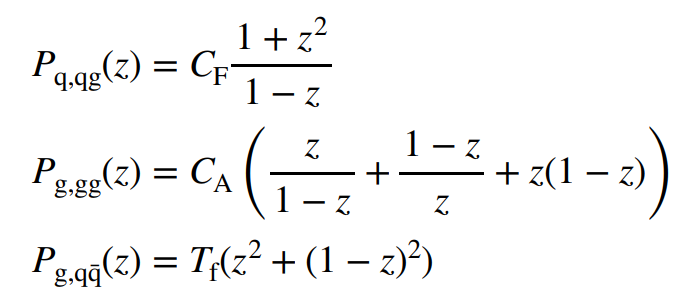
\includegraphics[width = 5 cm]{plots/AP_splitting.png}
		\end{figure}
		
		\column{0.6\textwidth}
		
		\begin{figure}
			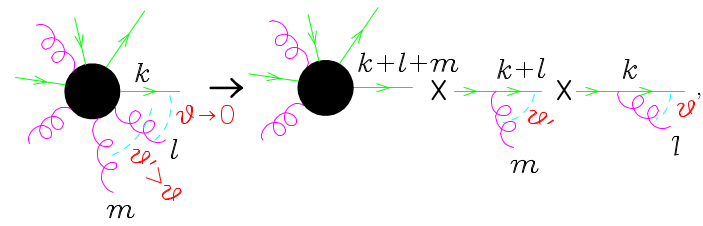
\includegraphics[width = 6.5 cm]{plots/AP_iteration_plot.png}
		\end{figure}

	\end{columns}

	\vspace{0.4cm}
	
	\footnotesize We can proceed in an iterative way	
	\begin{figure}
		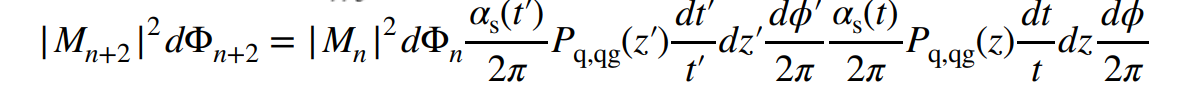
\includegraphics[width = 9 cm]{plots/AP_iteration_eq.png}
	\end{figure}

	\footnotesize Angles become, maintaining a strong ordering relation $\theta >> \theta' \rightarrow 0$
	
\end{frame}

% Parton showers V
\begin{frame}
	
	\frametitle{Parton showers}
	\framesubtitle{Exclusive final state}
	
	\footnotesize To describe exclusive final state $\rightarrow$ sum perturbative expansion to all orders in $\alpha_s$ \\
	
	\begin{figure}
		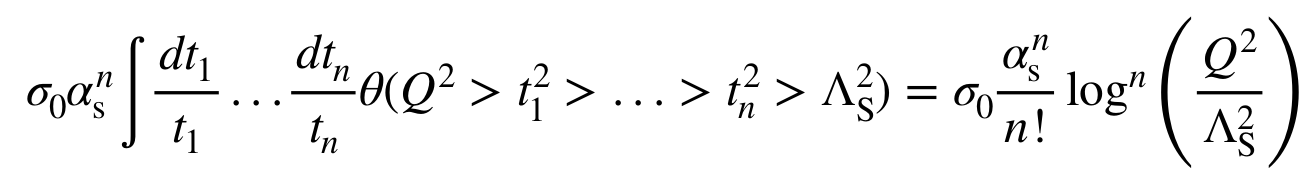
\includegraphics[width = 9 cm]{plots/exclusive_ll.png}
	\end{figure}
	
	\footnotesize Possible if we limit to the most singular terms, in ordered sequence of angles \\
	\color{red} Collinear approximation $\longrightarrow$ Leading log approximation

\end{frame}

% FSR I
\begin{frame}

	\frametitle{Final state radiation MC}
	\framesubtitle{General structure}
	
	\footnotesize Approximated description of a hadronic final state \\
	\footnotesize Model a given hard scattering with arbitrary number of enhanced radiations

	\begin{itemize} 
		\item Choose hard interaction with specified Born kinematics
		\item Consider all possible tree-level splittings for each coloured parton
		\item Assign the variables ($t, z, \phi$) at each splitting vertex, $t$ ordered in decreasing way.
		\item At each splitting vertex assign the weight 
		\begin{figure}
			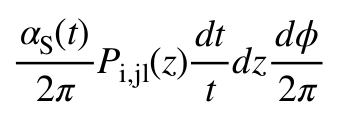
\includegraphics[width = 2.5 cm]{plots/AP_weight.png}
		\end{figure}
		\item Each line has a weight known as Sudakov factor
		\begin{figure}
			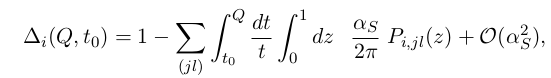
\includegraphics[width = 7 cm]{plots/sudakov.png}
		\end{figure}
	\end{itemize}

\end{frame}

% FSR II - Formal representation of a shower
\begin{frame}

	\frametitle{Final state radiation MC}
	\framesubtitle{Formal representation of a shower}
	
	\footnotesize Graphical notation for the representation of a shower \\
	
	\begin{columns} 
		
		\column{0.5\textwidth}
		
		\begin{figure}
			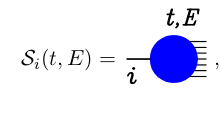
\includegraphics[width = 2.5 cm]{plots/shower_1.png}
		\end{figure}

		\column{0.5\textwidth}
		
		\footnotesize Ensemble of all possible branchings from parton $i$ at scale $t$

	\end{columns}

	\begin{figure}
		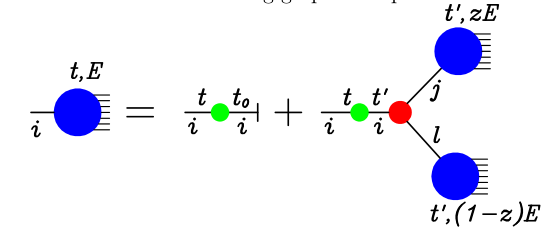
\includegraphics[width = 6 cm]{plots/shower_2.png}
	\end{figure}
		
	\footnotesize Forward evolution equation $\rightarrow$ recursive structure
	\begin{figure}
		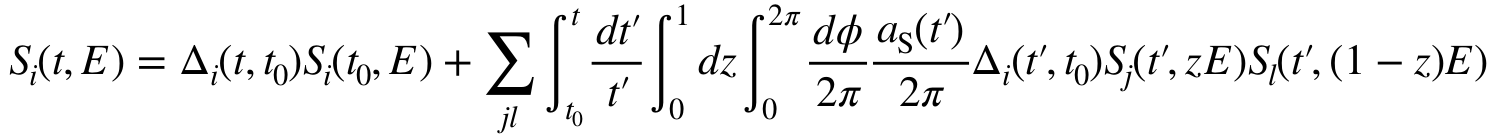
\includegraphics[width = 10 cm]{plots/shower_2_eq.png}
	\end{figure}

\end{frame}

% FSR III - Probabilistic interpretation
\begin{frame}

	\frametitle{Final state radiation MC}
	\framesubtitle{Probabilistic interpretation}

	\begin{columns} 
	
		\column{0.3\textwidth}
		
		\begin{figure}
			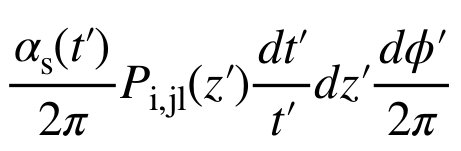
\includegraphics[width = 2.5 cm]{plots/probability1.png}
		\end{figure}
		
		\column{0.7\textwidth}
		
		\footnotesize Probability of branching in the infinitesimal volume $dt'\; dz\; d\phi$

	\end{columns}

	\begin{columns} 
	
		\column{0.5\textwidth}
		
		\begin{figure}
			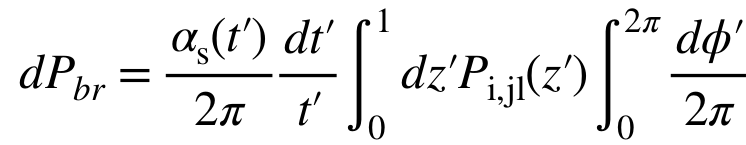
\includegraphics[width = 4 cm]{plots/probability2.png}
		\end{figure}
		
		\column{0.5\textwidth}
		
		\footnotesize Probability of branching in the interval dt'

	\end{columns}

	\begin{columns} 
	
		\column{0.6\textwidth}
		
		\begin{figure}
			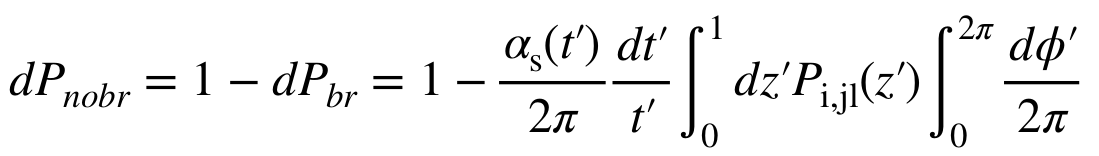
\includegraphics[width = 5.5 cm]{plots/probability3.png}
		\end{figure}
		
		\column{0.4\textwidth}
		
		\footnotesize Probability of first branching in the infinitesimal volume $dt'$
	
	\end{columns}

	\begin{columns} 
	
	\column{0.6\textwidth}
	
	\begin{figure}
		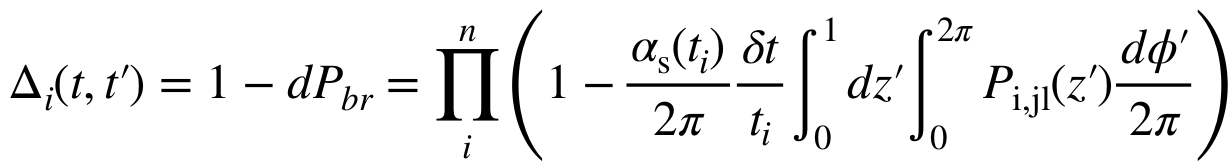
\includegraphics[width = 6 cm]{plots/probability4.png}
	\end{figure}
	
	\column{0.4\textwidth}
	
	\footnotesize Sudakov form factor from unitarity
	
	\end{columns}
	
	\begin{columns} 
		
		\column{0.4\textwidth}
		
		\begin{figure}
			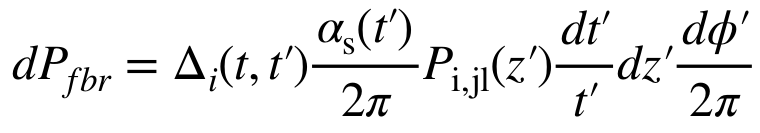
\includegraphics[width = 4 cm]{plots/probability5.png}
		\end{figure}
		
		\column{0.6\textwidth}
		
		\footnotesize Probability of no-branching in the infinitesimal volume $dt'\; dz\; d\phi$
		
	\end{columns}

\end{frame}

% FSR IV - Shower algorithm
\begin{frame}

	\frametitle{Final state radiation MC}
	\framesubtitle{Shower algorithm}
	
	\footnotesize Generate hard process with probability proportional to its parton level cross section. \\
	\footnotesize For each final state colored parton:
	\begin{enumerate} 
		\item \footnotesize Set scale $t = Q$, hard scale of the process.
		\item \footnotesize Generate random number $0 < r < 1$.
		\item \footnotesize Solve $r = \Delta_{i}(t, t')$ for $t'.$
		\item \footnotesize i) if $t' < t_{0}$, no further branching and stop shower.
		\item \footnotesize ii) if $t' \geq t_{0}$, generate $j, l$ with energies $$E_{j} = zE_{i} \quad \textrm{and}\quad E_{l} = (1 - z)E_{i}, $$ following the $P_{i, jl}(z)$ distribution and with azimuth $\phi$ uniform in the interval $[0, 2\pi]$. \\
		the angle of between their momenta is fixed by $t'$.
		\item \footnotesize For each branched partons set $t = t'$ and start from (2).
	\end{enumerate}

\end{frame}

% ISR I
\begin{frame}

	\frametitle{Initial state radiation MC}
	\framesubtitle{General structure}
	
	\center \footnotesize ISR showers are spacelike
	\begin{columns}
		
		\column{0.3\textwidth}
		
		\begin{figure}
			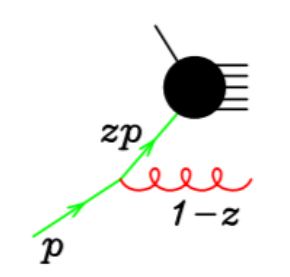
\includegraphics[width = 2 cm]{plots/ISR_shower0.png}
		\end{figure}
	
		\column{0.6\textwidth}
		
		\begin{figure}
			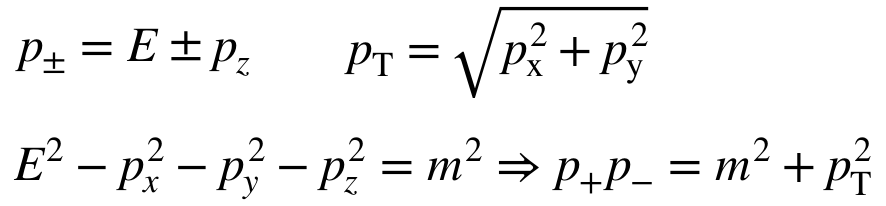
\includegraphics[width = 5 cm]{plots/ISR_spacelike.png}
		\end{figure}
		
	\end{columns}

	\vspace{0.5cm}
	\footnotesize Consider the splitting between a particle a that splits into b and c
	
	\begin{figure}
		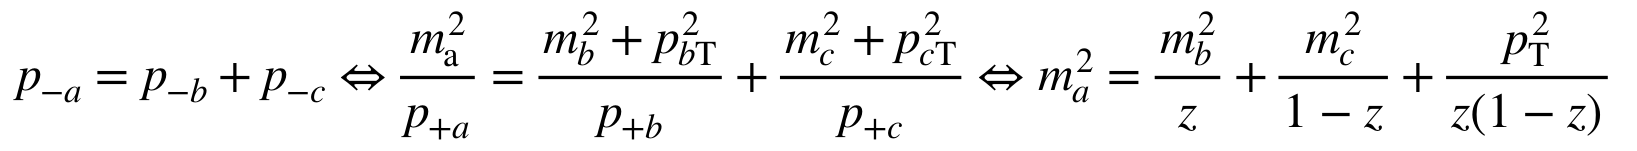
\includegraphics[width = 9 cm]{plots/ISR_splitting.png}
	\end{figure}

	\begin{figure}
		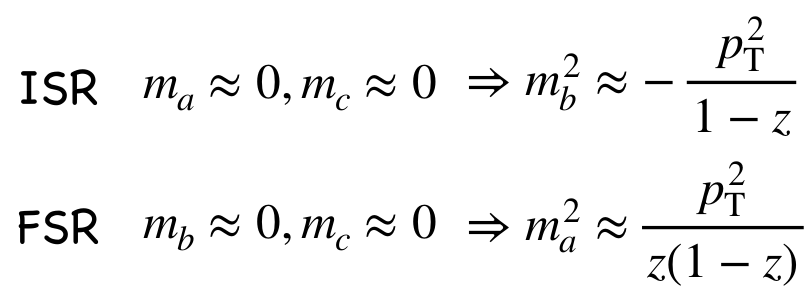
\includegraphics[width = 4.5 cm]{plots/ISR_FSR.png}
	\end{figure}

\end{frame}

% ISR II
\begin{frame}
	
	\frametitle{Initial state radiation MC}
	\framesubtitle{Formal representation}
	
	\begin{figure}
		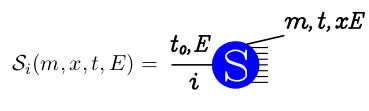
\includegraphics[width = 4 cm]{plots/shower_ISR_1.png}
	\end{figure}
	
	\begin{itemize} 
		\item \footnotesize Lines between $t_{1}$ and $t_{2}$ (consecutive radiations) are spacelike {\color{blue}(*)}
		\item \footnotesize Difference in Sudakov factors and Splitting functions start at NLO
	\end{itemize}
	
	\footnotesize Forward evolution equation. Great amount of computation time to generate configurations leading to the scattering that we want
	\begin{figure}
		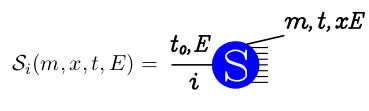
\includegraphics[width = 8.5 cm]{plots/shower_ISR_2.png}
	\end{figure}

\end{frame}

% ISR MC III
\begin{frame}

	\frametitle{Initial state radiation MC}
	\framesubtitle{Shower algorithm}
	
	\footnotesize Generate hard process with probability proportional to its parton level cross section.
	\footnotesize For each final state colored parton:
	\begin{enumerate} 
		\item Set scale $t = Q$, hard scale of the process.
		\item Generate random number $0 < r < 1$
		\item Solve $$r = \frac{f^{(i)}_{m} \Delta_{m}(t, t')}{f^{(i)}_{m}(t, x)} \quad \textrm{for }t'.$$
		\item i) if $t' < t_{0}$, no further branching and stop shower.
		\item \footnotesize ii) if $t' \geq t_{0}$, generate $j, l$ with energies $$E_{j} = zE_{i} \quad \textrm{and}\quad E_{l} = (1 - z)E_{i}, $$ following the $P_{i, jl}(z)$ distribution and with azimuth $\phi$ uniform in the interval $[0, 2\pi]$. \\
		the angle of between their momenta is fixed by $t'$.
		\item For parton $j$ set $t = t'$ and start from (2). For parton $l$ generate a timelike parton shower according to the algorithm shown previously.
	\end{enumerate}

\end{frame}

% Hadronization I
\begin{frame}
	
	\frametitle{Hadronization}
	\framesubtitle{Basics}

	\footnotesize A parton becoming a measurable hadron through the emission of a partonic shower \\
	\footnotesize Large number of color approximation $\rightarrow$ each parton identified by a unique label \\

	\begin{figure}
		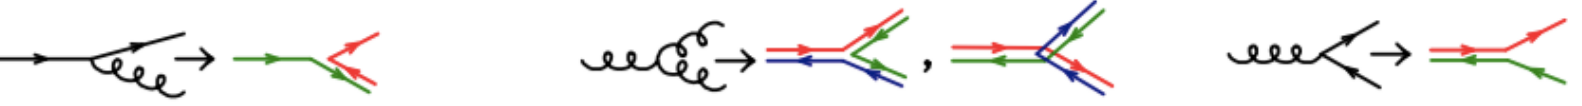
\includegraphics[width = 8.5 cm]{plots/hadronization.png}
	\end{figure}

	\footnotesize Hadronization models
	\begin{itemize}
		\item Lund string model
		\begin{itemize}
			\item \footnotesize non perturbative production of quarks and antiquarks
			\item \footnotesize intermediate gluons are transverse kicks of a continuum medium
		\end{itemize}
		\item Cluster models
		\begin{itemize}
			\item \footnotesize preconfinement, assuming subsystems of color singlet partons
			with universal invariant mass distribution (power suppressed at high masses)
			\item gluons are forced to split in quark-antiquark pair
		\end{itemize}
	\end{itemize}

\end{frame}

% Summary
\begin{frame}

	\frametitle{Summary}

\begin{itemize}
	\item \footnotesize LHC processes require factorization in perturbative and non perturbative part
	\item \footnotesize pQCD applied at high energies
	\item \footnotesize Monte Carlo shower programs describe non perturbative physics in hadron physics
	\item \footnotesize Agreement and precision Monte Carlo shower programs
\end{itemize}

\end{frame}

\end{document}